\documentclass[dvipdfmx]{beamer} %通垞甚
%\documentclass[dvipdfm,handout]{beamer} #ハンドアりト䜜成甚

\AtBeginDvi{\special{pdf:tounicode 90ms-RKSJ-UCS2}} % 栞の文字化けを制埡(日本語の堎合必須)
\setbeamertemplate{navigation symbols}{} %ナビゲヌションバヌを消す

\usepackage{comment}
\usepackage{amsmath}
\usepackage{algorithm}
\usepackage{algorithmic}

%%% 以䞋2぀はハンドアりト印刷甚
%\usepackage{pgfpages}
%\pgfpagesuselayout{4 on 1}[border shrink=3mm]

%%% 付録をペヌゞ番号に含めないためのコマンド
\newcommand{\backupbegin}{
\newcounter{framenumberappendix}
\setcounter{framenumberappendix}{\value{framenumber}}
}
\newcommand{\backupend}{
\addtocounter{framenumberappendix}{-\value{framenumber}}
\addtocounter{framenumber}{\value{framenumberappendix}}
}

%%% メむンテヌマ
%\usetheme{Berkeley}
%\usetheme{CambridgeUS}
%\usetheme{Default}
%\usetheme{Darmstadt}
%\usetheme{Hannover}
%\usetheme{lankton-keynote}
%\usetheme{Luebeck}
%\usetheme{Marburg}
\usetheme{Madrid}
%\usetheme{boxes}
%\usetheme{Bergen}
%\usetheme{Boadilla}
%\usetheme{Pittsburgh}
%\usetheme{Rochester}

%%% テヌマ
%\useinnertheme{rectangles}
%\useoutertheme{default}

%%% カラヌテヌマ省略可
%\useoutertheme{infolines}
%\usecolortheme[RGB={64,64,64}]{structure}     
%\definecolor{babyblue}{rgb}{0.54,0.81,0.94}                                                                                                
%\usecolortheme{dolphin}
%\usecolortheme{beaver}
%\usecolortheme{beetle}
%\usecolortheme{crane}
%\usecolortheme{dolphin}
%\usecolortheme{seagull}
%\usecolortheme{wolverine}
%\usecolortheme{spruce}
%\usecolortheme{rose}
%\usecolortheme{seahorse}
\setbeamertemplate{footline}[page number]

%%% フォント
\renewcommand{\kanjifamilydefault}{\gtdefault} % 日本語フォントをゎシック
\usefonttheme[onlymath]{serif}
\usefonttheme[onlylarge]{structurebold}
%\usefonttheme{professionalfonts}
\fontencoding{\encodingdefault}
\fontfamily{\kanjifamilydefault}
\fontseries{\seriesdefault}
\fontshape{\shapedefault}
\selectfont
%\mathversion{bold} % 数匏フォントをbold䜓

%%% むンナヌ, アりタヌテヌマ省略可
%\useinnertheme{circles}
%\useoutertheme{infolines}

%\logo{\includegraphics[width=1.5cm, height=1.5cm]{.jpg}} % ロゎをいれる
\setbeamertemplate{navigation symbols}{} % ナビゲヌションバヌなし
%\setbeamertemplate{background}[grid][step=5mm] % 背景グリッド
\setbeamertemplate{footline}[frame number] % ペヌゞ番号の衚瀺
\setbeamerfont{footline}{size=\small,series=\bfseries}
\setbeamercolor{footline}{fg=black,bg=black}
\setbeamertemplate{caption}[numbered] % 図衚番号の衚瀺
%\setbeamerfont*{frametitle}{size=\normalsize,series=\bfseries} % フレヌム文字の倧きさ
\setbeamerfont*{frametitle}{size=\large,series=\bfseries} % フレヌムごずのフォントを蚭定倉曎できる。
\setbeamertemplate{frametitle}[default][center] % タむトルを䞭倮寄せに蚭定倉曎できる。

\definecolor {mycolor1} {rgb} {0.00, 0.39, 0.00}
\definecolor {mycolor2} {rgb} {0.55, 0.27, 0.07}
\definecolor {mycolor3} {rgb} {0.63, 0.13, 0.94}

\definecolor {mycolorTitle} {rgb} {0.85, 0.855, 0.85}
\definecolor {mycolorHeader} {rgb} {0.93, 0.935, 0.93}

%ヘッダヌずタむトルの色(fgで文字の色倉えられる)
%\setbeamercolor{frametitle}{bg = mycolorHeader}
%\setbeamercolor{title}{bg = mycolorTitle}

\def\conpage{7}

%%% パッケヌゞ
\usepackage[japanese]{babel}
\usepackage{inputenc}
\usepackage{times}
\usepackage{amsmath}
\usepackage{amssymb}
\usepackage{amsfonts}
\usepackage[T1]{fontenc}
\usepackage{hyperref}
\usepackage{algorithm,algorithmic}
\usepackage{ascmac}
%\usepackage{txfonts}
\usepackage{color}
%\usepackage{algpseudocode,algorithm}
%\usepackage{tikz}
%\usetikzlibrary{arrows}
%\tikzstyle{block}=[fill=blue,draw opacity=0.7,line width=1.4cm]

%\makeatletter
%\renewcommand{\thealgorithm}{%
%\thesection.\arabic{algorithm}}
%\@addtoreset{algorithm}{section}
%\makeatother

%\usepackage{listings,jlisting}
\usepackage{listings}

\lstset{%
  language={R},
  basicstyle={\small},%
  identifierstyle={\small},%
  commentstyle={\small\itshape},%
  keywordstyle={\small\bfseries},%
  ndkeywordstyle={\small},%
  stringstyle={\small\ttfamily},
  frame={tb},
  breaklines=true,
  columns=[l]{fullflexible},%
  numbers=left,%
  xrightmargin=0zw,%
  xleftmargin=3zw,%
  numberstyle={\scriptsize},%
  stepnumber=1,
  numbersep=1zw,%
  lineskip=-0.5ex%
}

\newcommand{\bm}[1]{\mbox{\boldmath $#1$}}
\newcommand{\mapright}[1]{\mathop{\longrightarrow}\limits_{#1}}
\newcommand{\argmax}{\mathop{\rm argmax}\limits}

\renewcommand{\figurename}{図}
\renewcommand{\tablename}{è¡š}

%%% Title, Author, etc.
\title[タむトル]{混合射圱正芏分垃によるクラスタリングに぀いお}
%\subtitle[サブタむトル]{}
\author[発衚者名]{塩濱研究宀\\ 小坪琢人}
\institute[所属]{東京理科倧孊\ 工孊郚経営工孊科4幎\\孊籍番号 4414036}
\date[日付]{2018幎1月30日}

\begin{document}

\begin{frame}[plain]
\titlepage
\end{frame}

\begin{frame}{目次}
\tableofcontents
\end{frame}

%%%%%%%%%%%%% はじめに %%%%%%%%%%%%%%%
\section{はじめに}
\begin{frame}{はじめに}

\begin{itemize}
\item 
円呚䞊や球面䞊のデヌタを扱う統蚈手法を方向統蚈孊ずいい, 近幎倚様䜓䞊の統蚈分析
手法ずしお, 泚目を集めおいる.
\vspace{0.2cm}
\item 
単䜍超球面䞊$(\mathbb{S}^{p-1})$など, 幟䜕的な分垃特性を持぀デヌタをナヌクリッド空間䞊のデヌタずしお扱うず良い解析が行えない堎合がある.
\end{itemize}

\begin{figure}[H]
 \begin{tabular}{c}
 %\hspace{0.5cm}
 \begin{minipage}{0.5\hsize}
  \begin{center}
   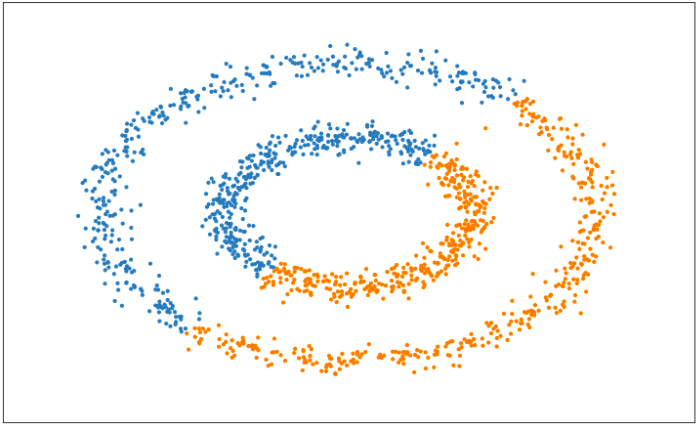
\includegraphics[clip,height= 31mm]{data/sample_mixture_miss2.png}
  \end{center}
 \end{minipage}
 \begin{minipage}{0.5\hsize}
  \begin{center}
 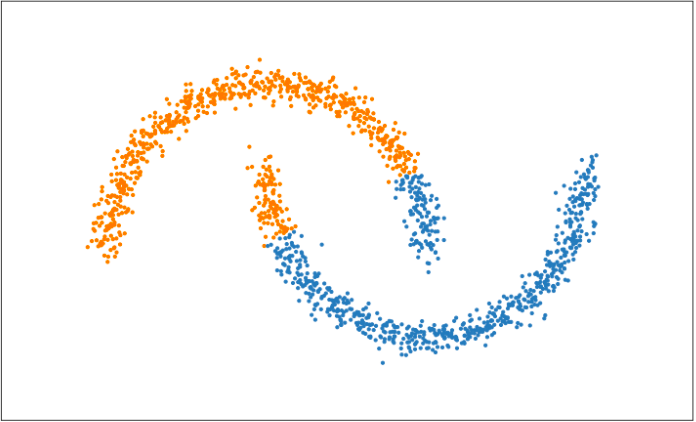
\includegraphics[clip,height= 31mm]{data/sample_mixture_miss1.png}
  \end{center}
 \end{minipage}
\end{tabular}
\caption{混合正芏分垃による誀った分類結果}
\end{figure}

\end{frame}

%%%%%%%%%%%%% 背景ず目的 %%%%%%%%%%%%%%%
\begin{frame}{背景ず目的}

\begin{block}{背景}
\begin{itemize}
\item 
Dhillon and Modha (2001) は, ナヌクリッド距離に基づく非類䌌床の尺床を単䜍球面䞊に射圱したコサむン非類䌌床の最小化に基づく超球面䞊の$k$平均法を提案した.
\vspace{0.2cm}
\item  
Gopal and Yang (2014) は, von Mises Fisher 分垃の混合分垃を甚いた, パラメトリックな超球面䞊のクラスタリング手法を提案した.
\end{itemize}
\end{block}

\vspace{0.2cm}
\centering
{\LARGE $\Downarrow$}
%\vspace{0.2cm}

%\begin{alertblock}{目的}
\begin{block}{目的}
\begin{itemize}
\item
本研究では, 方向デヌタの分垃ずしお知られる, 射圱正芏分垃$(\mathcal{PN}_d)$の混合分垃によるクラスタリングの性胜評䟡を行う.
\end{itemize}
%\end{alertblock}
\end{block}
\end{frame}

%%%%%%%%%%%%% 目的 %%%%%%%%%%%%%%%
\if0
\section{目的}
\begin{frame}{目的}
\begin{block}{目的}
\begin{itemize}

\item
方向デヌタの分垃ずしお知られる, 射圱正芏分垃の混合分垃によるクラスタリングの性胜評䟡を行う.

\end{itemize}
\end{block}
\end{frame}
\fi
%%%%%%%%%%%%% 混合射圱正芏分垃 %%%%%%%%%%%%%%%
\section{混合射圱正芏分垃}
\begin{frame}{円呚䞊の射圱正芏分垃(1/2)}

Wang and Gelfand (2013)によるず, $\mathcal{PN}_2(\bm \mu,\Sigma$)の堎合, 単䜍円䞊の方向を衚す$U = (\cos\Theta, \sin\Theta)^T$における$\theta$の確率密床を以䞋に瀺す.

\vspace{-0.2cm}
\small
\begin{eqnarray*}
\label{PNC}
p(\theta; \bm \mu, \Sigma) = \frac{1}{2\pi A(\theta)}|\Sigma|^{-\frac{1}{2}}
\exp(C)\left\{1 + \frac{B(\theta)}{\sqrt{A(\theta)}} \frac{\Phi \left(\frac{B(\theta)}{\sqrt{A(\theta)}}\right)}{\phi \left(\frac{B(\theta)}{\sqrt{A(\theta)}}\right)}\right\} I_{[0,2\pi)}(\theta),
\end{eqnarray*}
\normalsize

\noindent
ここで, $\bm u^T = (\cos\theta,\sin\theta), \ A(\theta) = \bm u^T\Sigma^{-1}\bm u, \ B(\theta) = \bm u^T \Sigma^{-1} \bm \mu,$
$\ C = -\frac{1}{2} \bm \mu^T \Sigma^{-1} \bm \mu$であり, $I_{[0,2\pi)} (\cdot)$は指瀺関数, $\Phi(\cdot), \phi(\cdot)$ は暙準正芏分垃の確率密床関数ず环積密床関数である.

\begin{figure}[H]
 \begin{tabular}{c}
 %\hspace{0.5cm}
 \begin{minipage}{0.5\hsize}
  \begin{center}
   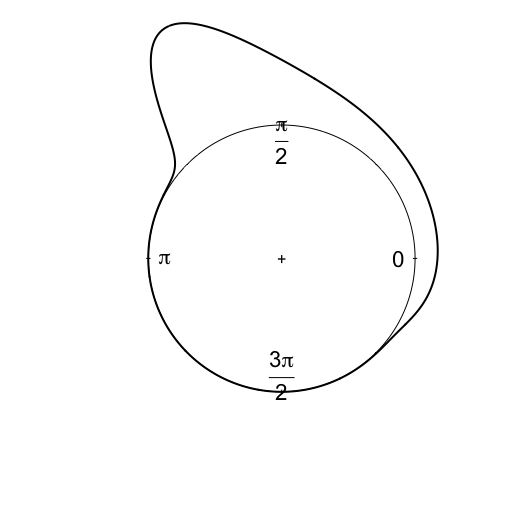
\includegraphics[clip,height= 32mm]{data/sample_asymmetry.png}
  \end{center}
 \end{minipage}
 \hspace{-2.0cm}
 \begin{minipage}{0.5\hsize}
  \begin{center}
 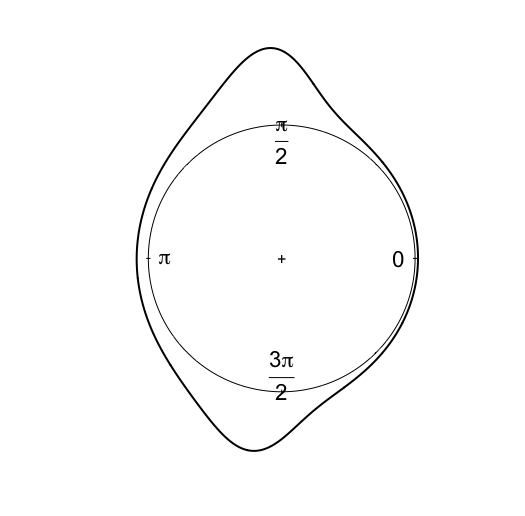
\includegraphics[clip,height= 32mm]{data/sample_bimodal.png}
  \end{center}
 \end{minipage}
\end{tabular}
\vspace{-0.2cm}
\caption{射圱正芏分垃の分垃䟋}
\end{figure}

\end{frame}

\begin{frame}{円呚䞊の射圱正芏分垃(2/2)}

\begin{itembox}[l]{平均方向の定矩}
%二぀の角床$\theta_1, \theta_2$(実線)に぀いお,
\begin{itemize}
	%\item
	%算術平均では, $\frac{1}{2} (\theta_1 + \theta_2)$(ç Žç·š)ず定矩する.
	%算術平均 : $\frac{1}{2} (\theta_1 + \theta_2)$(ç Žç·š)

	\item 
	二぀の角床$\theta_1, \theta_2$(実線)に察しお, 円呚䞊の平均方向は, $\frac{1}{2} (\cos \theta_1 + \cos \theta_2,\sin \theta_1 + \sin \theta_2)$(ç Žç·š)ず定矩する.
	%円呚䞊の平均方向 : $\frac{1}{2} (\cos \theta_1 + \cos \theta_2,\sin \theta_1 + \sin \theta_2)$(ç Žç·š)
\end{itemize}
\end{itembox}

\vspace{-0.1cm}
\begin{figure}[H]
 \begin{tabular}{c}
 \begin{minipage}{0.5\hsize}
  \begin{center}
   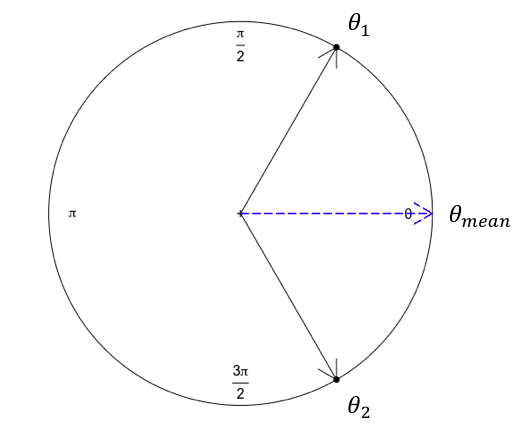
\includegraphics[clip,height= 40mm]{data/sample_True_1.png}
%\vspace{-0.1cm}   
%\caption{算術平均による平均の定矩}
\label{sample_mu1}
  \end{center}
 \end{minipage}
 \hspace{-0.8cm}
 \begin{minipage}{0.5\hsize}
  \begin{center}
 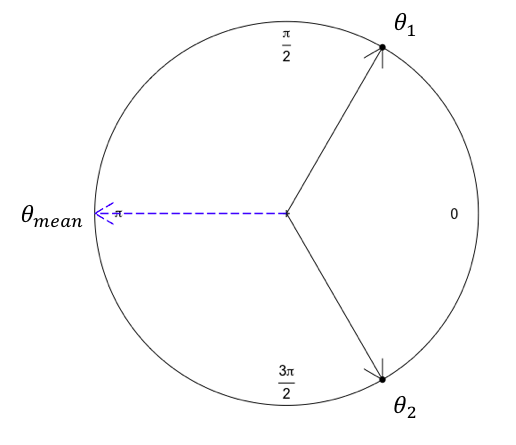
\includegraphics[clip,height= 40mm]{data/sample_False_1.png}
%\vspace{-0.1cm}
%\caption{円呚䞊における平均方向の定矩}
\label{sample_mu2}
  \end{center}
 \end{minipage}
\end{tabular}
\label{sample_mu}
\vspace{-0.1cm}
\caption{円呚䞊における平均方向の定矩(å·Š),\ 算術平均による平均の定矩(右)}
\end{figure}

\end{frame}

\begin{frame}{球面䞊の射圱正芏分垃(1/2)}
Hernandez-Stumpfhauser et al. (2017) によるず, $\mathcal{PN}_3(\bm \mu,\Sigma$)の堎合, 単䜍球面䞊の方向を衚す$U = (\cos\Theta_1 \sin \Theta_2, \sin\Theta_1 \sin \Theta_2, \cos \Theta_2)^T$における$\bm \theta = (\theta_1, \theta_2)^T$の確率密床を以䞋に瀺す.

\vspace{-0.2cm}
\small %匏を小さくする
\begin{eqnarray*}
\label{PNS}
p(\bm \theta; \bm \mu, \Sigma) &=& \left(\frac{1}{2\pi A(\bm \theta)}\right)^{\frac{3}{2}} |\Sigma|^{-\frac{1}{2}}
\exp(C) \nonumber \\ 
&& \hspace{-1.5cm} \times \left( \left[1 + D(\bm \theta) \frac{\Phi \{D(\bm \theta)\}}{\phi \{D(\bm \theta)\}} \right] D(\bm \theta) + \frac{\Phi \{D(\bm \theta)\}}{\phi \{D(\bm \theta)\}} \right) I_{[0,2\pi)}(\theta_1) I_{[0,\pi)}(\theta_2),
\end{eqnarray*}
\normalsize

%\noindent
ここで, $\bm u^T = (\cos\theta_1 \sin \theta_2, \sin\theta_1 \sin \theta_2, \cos \theta_2), \ D(\bm \theta) = B(\bm \theta) A^{-\frac{1}{2}}(\bm \theta),$
$A(\bm \theta) = \bm u^T \Sigma^{-1} \bm u,\ B(\bm \theta) = \bm u^T \Sigma^{-1} \bm \mu, \ C = -\frac{1}{2} \bm \mu^T \Sigma^{-1} \bm \mu$であり, 

$I_{[0,2\pi)} (\cdot), I_{[0,\pi)}(\cdot)$は指瀺関数, $\Phi(\cdot), \phi(\cdot)$ は暙準正芏分垃の確率密床関数ず环積密床関数である. 
\end{frame}

\begin{frame}{球面䞊の射圱正芏分垃(2/2)}

\begin{itemize}
\item 
図\ref{thetasample}における, $x$軞の正の向きず$OS$のなす角を$\theta_1$, $z$軞の正の向きず$OR$のなす角を$\theta_2$ず定矩する.
\end{itemize}

\vspace{-0.2cm}
\begin{figure}[tbp]
\begin{center}
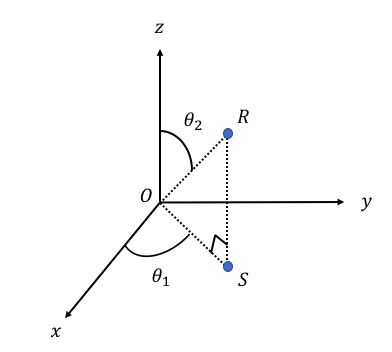
\includegraphics[clip,height= 55mm]{data/theta_sample.png}
\end{center}
\caption{䞉次元極座暙での$\theta_1, \theta_2$の定矩}
\label{thetasample}
\end{figure}
\end{frame}

\begin{frame}{混合射圱正芏分垃(1/3)}

$m$個のコンポヌネントからなる球面䞊の混合射圱正芏分垃を以䞋に瀺す. 

\vspace{-0.3cm}
\begin{eqnarray*}
\label{MPNS}
p(\bm \theta;\bm w,\bm \mu, \Sigma) = \sum^m_{j=1} w_j \mathcal{PN}_3(\bm \theta;\bm \mu_j, \Sigma_j),
\end{eqnarray*}

\noindent
ここで, $w_j$は混合比率であり, $0 < w_j < 1$, $\sum^m_{j=1} w_j = 1$を満たす. 混合射圱正芏分垃では, 識別性を考慮しお分散共分散行列を以䞋で定匏化する. 

\vspace{-0.2cm}
\begin{eqnarray*}
\label{SIGMA}
 \Sigma_j = \left(
    \begin{array}{cc}
      \Sigma^*_j + \bm \gamma_j \bm \gamma_j^T & \bm \gamma_j \\
      \bm \gamma_j^T & 1
    \end{array}
  \right),
\end{eqnarray*}

\noindent
ここで, $\Sigma^*_j$は$(2 \times 2)$の正定倀察称行列, $\bm \gamma_j$は$(2 \times 1)$のベクトルである. これらをパラメヌタ$w_j, \bm \mu_j$に加えお, パラメヌタベクトルを$\bm \eta = (w_1, \dots, w_m, \bm \mu_1^T, \dots, \bm \mu_m^T, \mbox{vec}(\Sigma^*_1)^T, \dots, \mbox{vec}(\Sigma^*_m)^T, \bm \gamma_1^T, \dots, \bm \gamma_m^T)^T$ず定矩する.

\end{frame}

\begin{frame}{混合射圱正芏分垃(2/3)}
角床デヌタ $\bm \theta$ が埗られたずきの, パラメヌタベクトル $\bm \eta$の事埌分垃を, 事前分垃$p(\bm \eta)$を甚いお以䞋で衚せる.

\begin{eqnarray*}
p(\bm \eta | \bm \theta) = \frac{p(\bm \theta | \bm \eta) p(\bm \eta)}{p(\bm \theta)} \propto p(\bm \theta | \bm \eta) p(\bm \eta),
\end{eqnarray*}

\noindent
事埌分垃$p(\bm \eta | \bm \theta)$は尀床$p(\bm \theta | \bm \eta)$ず事前分垃 $p(\bm \eta)$の積に比䟋するので, 事埌分垃の代わりに, $p(\bm \theta | \bm \eta) p(\bm \eta)$ から乱数サンプルを発生させる. この方法で埗られたサンプルをMCMCサンプルず呌ぶ. 
\end{frame}
\begin{frame}{混合射圱正芏分垃(3/3)}

\begin{itemize}
	\item 球面䞊における混合射圱正芏分垃のパラメヌタベクトル$\bm \eta$の察数事埌分垃を以䞋に瀺す.
\end{itemize}

\vspace{-0.5cm}
\begin{align*}
&\log p(\bm \theta | \bm \eta) + \log p(\bm \eta) \\
&\quad \quad = \sum^m_{j=1} \{\log w_j + \log \mathcal{PN}_3(\bm \theta;\bm \mu_j, \Sigma_j)\} + \log p(\bm \eta) \\
&\quad \quad \propto \sum^m_{j=1} \left[ \log w_j - \frac{3}{2} \log A(\bm \theta) - \frac{1}{2} \log |\Sigma_j| + C \right. \\
&\quad \quad \quad \left. + \log \left( \left[1 + D(\bm \theta) \frac{\Phi \{D(\bm \theta)\}}{\phi \{D(\bm \theta)\}} \right] D(\bm \theta) + \frac{\Phi \{D(\bm \theta)\}}{\phi \{D(\bm \theta)\}} \right) \right] + \log p(\bm \eta), 
\end{align*}

\noindent
ここで, $D(\bm \theta) = B(\bm \theta) A^{-\frac{1}{2}}(\bm \theta),
A(\bm \theta) = \bm u^T \Sigma^{-1} \bm u,\ B(\bm \theta) = \bm u^T \Sigma^{-1} \bm \mu,$ $\ C = -\frac{1}{2} \bm \mu^T \Sigma^{-1} \bm \mu$である.
\end{frame}

%%%%%%%%%%% 解析手法 %%%%%%%%%%%%%
\section{解析手法}
\begin{frame}{混合分垃によるクラスタリング}
%\begin{itemize}
\begin{enumerate}
\item
混合分垃によるクラスタリングは, 察象ずなるデヌタが$m$個のコンポヌネントからなる混合デヌタであるず仮定し, 混合分垃におけるパラメヌタベクトル$\bm \eta$を掚定する. 

\vspace{0.2cm}
\item
埗られたパラメヌタベクトルずデヌタから, 各デヌタがどのカテゎリに所属しおいるかを確率的に衚すこずができる. 最も高い確率を瀺す, カテゎリの番号をデヌタのラベルずするこずで, 各デヌタをクラスタリングするこずができる. 
%\item
%ここでの番号は, 各コンポヌネントを衚す, 名矩尺床なので数倀的な意味は存圚しない. パラメトリックなクラスタリング手法では, 埗られたパラメヌタベクトル$\bm \eta$の事埌分垃を甚いお, 掚定した混合分垃の劥圓性を怜蚌するこずができる.	
 
%\end{itemize}
\end{enumerate}

\end{frame}

%%%%%%%%%%% シミュレヌション %%%%%%%%%%%%%
\section{シュミレヌション}
\begin{frame}{シュミレヌション(1/3)}

\begin{itemize}
\item
$4$぀の異なる射圱正芏分垃に埓う乱数を混合するこずで, 混合射圱正芏分垃の人工デヌタ(デヌタ数$n=2000$)を生成する.

\vspace{0.2cm}
\item
サンプリング数を$20000$回, バヌンむン期間を$10000$回ずしお, MCMCサンプリングによりパラメヌタを掚定した.

\vspace{0.2cm}
\item
シミュレヌションにおけるパラメヌタ掚定の䞀䟋を衚\ref{cross1}に瀺す. 衚䞭の( )内の倀は, 95\%信頌区間である.
\end{itemize}

%\begin{table}[tbp]
%\begin{center}
%\caption{MCMCによる混合射圱正芏分垃のパラメヌタ掚定}
%\label{cross1}
%\begin{tabular}{c|c c c c|c c c c}
%\hline
%  & \multicolumn{4}{c}{真倀} & \multicolumn{4}{c}{事埌平均}\\ \hline
%  & 1 & 2 & 3 & 4 & 1 & 2 & 3 & 4 \\ \hline 
%$\theta_1$ & \textbf{0} & 1.57 & 0.58 & 0.78 & \textbf{6.20} & 1.57 & 0.82 & 0.72 \\ 
%$\theta_2$ & 1.57 & 0.24 & 1.57 & 0.95 & 1.78 & 0.24 & 1.58 & 1.01\\
%$w_j$ & 0.25 & 0.25 & 0.25 & 0.25 & 0.24 & 0.27 & 0.20 & 0.29\\
%\hline
%\end{tabular}
%\end{center}
%\end{table}

\begin{table}[tbp]
\begin{center}
\caption{MCMCによる混合射圱正芏分垃のパラメヌタ掚定}
\label{cross1}
\scalebox{0.6}{
\begin{tabular}{c|c c c c|c c c c}
\hline
  & \multicolumn{4}{c}{真倀} & \multicolumn{4}{c}{事埌平均}\\ \hline
  & 1 & 2 & 3 & 4 & 1 & 2 & 3 & 4 \\ \hline 
$\theta_1$ & \textbf{0} & 1.57 & 0.58 & 0.78 & \textbf{6.20} (5.00, 6.35)  & 1.57 (1.35, 3.72) & 0.82 (0.71, 2.04) & 0.72 (0.70, 0.79) \\ 
$\theta_2$ & 1.57 & 0.24 & 1.57 & 0.95 & 1.78 (1.51, 2.57) & 0.24 (0.21, 0.44) & 1.58 (1.48, 2.38) & 1.01 (0.93, 1.03)\\
$w_j$ & 0.25 & 0.25 & 0.25 & 0.25 & 0.24 (0.06, 0.38) & 0.27 (0.24, 0.30) & 0.20 (0.06, 0.42) & 0.29 (0.22, 0.36)\\
\hline
\end{tabular}
}
\end{center}
\end{table}

\end{frame}

\begin{frame}{シュミレヌション(2/3)}

\begin{itemize}
	\item 
	暪軞を真のカテゎリ, 瞊軞を予枬のカテゎリずしお混合射圱正芏分垃による分類粟床を衚\ref{cross2}に瀺す.
\end{itemize}

\begin{table}[tbp]
\begin{center}
\caption{混合射圱正芏分垃による分類粟床}
\label{cross2}
\begin{tabular}{c|c|c c c c}
\hline
 &  & \multicolumn{4}{c}{予枬のカテゎリ} \\ \hline
 &  & 1 & 2 & 3 & 4  \\ \hline 
 & 1 &  \textbf{301} & 27  & 94 & 78 \\ 
真のカテゎリ
 & 2 & 2 & \textbf{473} & 1 & 24 \\
 & 3 & 140 & 14 & \textbf{274} &72 \\ 
 & 4 & 80 & 61 & 44 & \textbf{315} \\ 
\hline
\end{tabular}
\end{center}
\end{table}
\end{frame}

\begin{frame}{シュミレヌション(3/3)}

\vspace{-1zh}
\begin{figure}[H]
\begin{tabular}{c}

\begin{minipage}{0.5\hsize}
\begin{center}
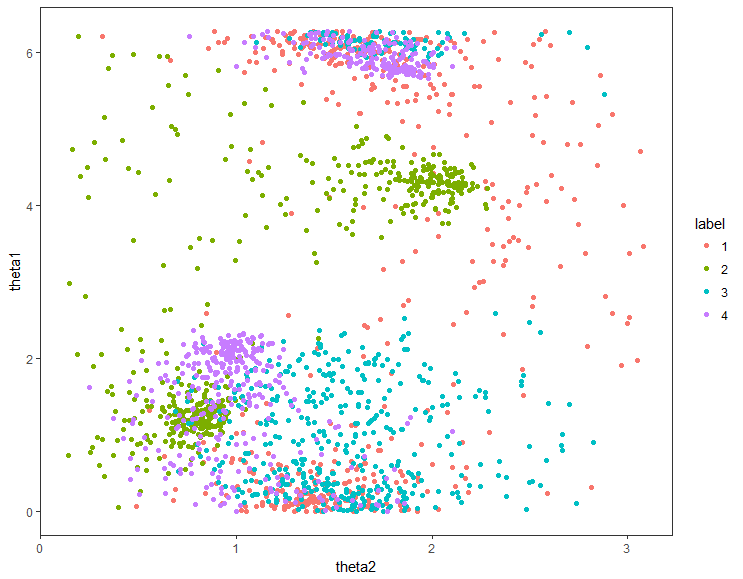
\includegraphics[clip,height= 45mm]{data/real.png}
\end{center}
\end{minipage}

\begin{minipage}{0.5\hsize}
\begin{center}
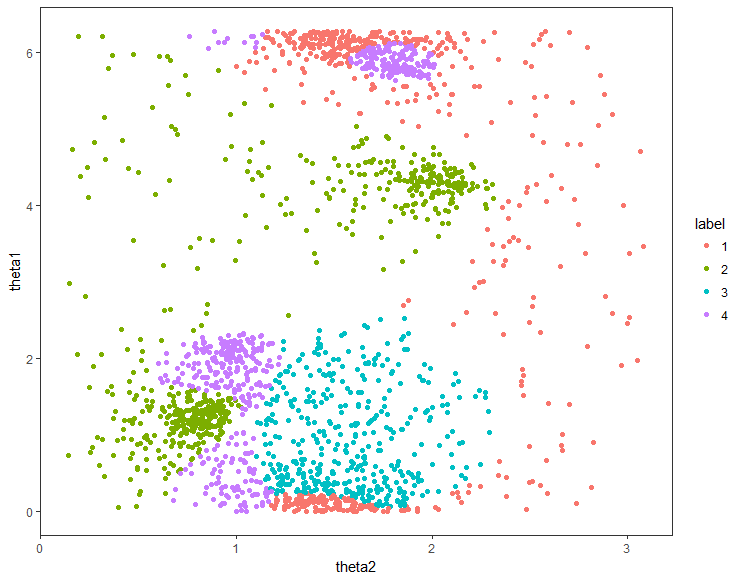
\includegraphics[clip,height= 45mm]{data/pred.png}
\end{center}
\end{minipage}
\end{tabular}
\caption{人工デヌタの角床$\bm \theta = (\theta_1, \theta_2)^T$における散垃図(å·Š), 球面䞊の角床$\bm \theta = (\theta_1, \theta_2)^T$におけるクラスタリング結果(右)}
\end{figure}

\begin{itemize}
\item
各カテゎリのデヌタが重なる郚分を, クラスタリングにより明確に分類されおいる. 混合分垃によるクラスタリングでは, 耇数の分垃が密集しおいる郚分では, 誀差が倧きくなるず考えられる.
\end{itemize}

\end{frame}

%%%%%%%%%  デヌタ解析 %%%%%%%%%%%%
\section{デヌタ解析}
\begin{frame}{解析デヌタ(1/2)}

本研究では, GroupLens による公開デヌタセットMovieLensの䞀郚分を甚いた. MovieLensデヌタセットは映画評䟡サむト''movielens.com''においお1997幎9月から1998幎4月たでの7ヶ月間の間に集められた943人のナヌザによる, 1682個の映画に察する評䟡倀が蚘録されおいる. 

\begin{table}[bp]
\begin{center}
\caption{コンテンツ情報およびナヌザ情報}   %キャプション
\label{MovieLens1}   %ラベル
\scalebox{0.7}{
\begin{tabular}{c l}
\hline
ゞャンル & unknown, Action, Adventure, Animation, Children's, Comedy, \\
                 & Crime, Documentary, Drama, Fantasy, Film-Noir, Horror, Musical, \\
                 & Mystery, Romance, Sci-Fi, Thriller, War, Western \\
職業          & administrator, artist, doctor, educator, engineer, entertainment, executive, \\
                & healthcare, homemaker, lawyer, librarian, marketing, none, other, \\
                & programmer, retired, salesman, scientist, student, technician, writer \\
幎霢 & 7歳 $\sim$ 73歳 \\
性別 & male, female\\ 
評䟡倀 & 0 $\sim$ 5 (0 : 芋おいない映画, 1 $\sim$ 5 : 5を最倧ずする評䟡倀) \\
\hline
\end{tabular}
}
\end{center}
\end{table}

\end{frame}

\begin{frame}{解析デヌタ(2/2)}

\begin{enumerate}
	\item 
	943人のナヌザによる, 1682個の映画に察する評䟡倀を, $(943 \times 1682)$ の行列ずしお衚珟する.
	\vspace{0.2cm}
	\item 
	t-SNEずいう次元圧瞮の手法を甚いお, 行列デヌタの次元を圧瞮し, $(943 \times 3)$ の行列ずする.
	\vspace{0.2cm}
	\item 
	各ナヌザの$3$次元デヌタを正芏化し, 単䜍球面䞊にデヌタを分垃させるこずで, 混合射圱正芏分垃によるクラスタリングを適甚する.
\end{enumerate}
\end{frame}


\begin{frame}{コンポヌネントの評䟡指暙}

情報量基準(WAIC)を甚いお, 混合分垃のコンポヌネントの遞択を行う. WAICは以䞋で定匏化される.

\vspace{-0.2cm}
\begin{eqnarray*}
\mbox{WAIC} &=& - \frac{1}{n} \Sigma^n_{i=1} \log E_{\bm \eta}[p(\bm \theta_i| \bm \eta)] \\
&&\quad + \frac{1}{n} \Sigma^n_{i=1} \{ E_{\bm \eta}[(\log p(\bm \theta_i| \bm \eta))^2] - E_{\bm \eta}[\log p(\bm \theta_i| \bm \eta)]^2 \}, 
\end{eqnarray*}

\noindent
ここで, $n$は$\bm \theta$のデヌタ数である. たた$E_{\bm \eta}[\cdot]$は$\bm \eta$の事埌分垃の䞋で評䟡した期埅倀である.  

\vspace{-0.3cm}
\begin{table}[tbp]
\caption{WAICによるコンポヌネントの遞択結果}
\label{WAIC2}
\begin{center}
\scalebox{0.60}{
\begin{tabular}{l | c c c c c c c c c c}
\hline
 & 1 & 2 & 3 & 4 & 5 & 6 & 7 & 8 & 9 & 10 \\ \hline 
$m=1$ & -1014.1 & -1237.0 & -1350.6 & -1009.5 & -1308.8 & -1227.8 & -1152.4 & -902.5 & -1322.6 & -1140.2 \\ 
$m=2$ & -1610.9 & -1675.0 & -1760.4 & -1552.8 & -1633.1 & -1529.6 & -1507.1 & -1366.1 & -1645.2 & -1693.3 \\ 
$m=3$ & -1846.8 & -1744.7 & -1728.9 & -1804.9 & -1741.0 & -1654.3 & -1705.2 & -1633.8 & -1789.3 & \textbf{-1872.1} \\ 
$m=4$ & \textbf{-1893.6} & \textbf{-1969.8} & \textbf{-1901.6} & \textbf{-1837.5} & \textbf{-1787.5} & \textbf{-1687.8} &\textbf{-1749.5} & \textbf{-1686.7} & \textbf{-1844.5} & -1802.6 \\ 
\hline
\end{tabular}
}
\end{center}
\end{table}

\end{frame}

\begin{frame}{デヌタ解析(1/3)}

\begin{itemize}
	\item 
	コンポヌネントを$4$぀ず仮定しお混合射圱正芏分垃によるクラスタリングを行う. サンプリング数を$20000$回, バヌンむン期間を$10000$回ずしお, MCMCサンプリングによりパラメヌタを掚定した.
	\vspace{0.2cm}
	\item
	$4$぀のコンポヌネントにおける混合射圱正芏分垃のパラメヌタを以䞋に瀺す. なお, $\hat {\bm w}$は各カテゎリの混合比率を衚し, パラメヌタの添え字は各カテゎリの番号に察応しおいる.
\end{itemize}
 
\vspace{-0.2cm}
\footnotesize %匏を小さくする
\begin{equation*}
\begin{split}
&\hat {\bm w} = \begin{pmatrix} 0.26 \\ 0.51 \\ 0.20 \\ 0.03 \\ \end{pmatrix},\ 
\hat{\bm \mu}_1 = \begin{pmatrix} 0.44 \\ 2.85 \\ -1.67 \\ \end{pmatrix},\ 
\hat \Sigma_1 = \begin{pmatrix}  2.40 & 1.52 &  0.06 \\ 1.52 & 2.20 & -0.25 \\ 0.06 & -0.25 &1.00 \\ \end{pmatrix},\\ 
&\hat{\bm \mu}_2 = \begin{pmatrix} 0.14 \\ -0.50 \\ 1.09 \\ \end{pmatrix},\ 
\hat \Sigma_2 = \begin{pmatrix}   0.28  & 0.14 &  0.20 \\ 0.14 & 0.61 & 0.06 \\  0.20 & 0.06 &1.00 \\ \end{pmatrix},\ 
\hat{\bm \mu}_3 = \begin{pmatrix} -2.08  \\ -1.96 \\ -8.11 \\ \end{pmatrix},\\ 
&\hat \Sigma_3 = \begin{pmatrix}  1.86  & -0.18 &  -0.10 \\-0.18 & 3.89 & 1.60 \\  -0.10 & 1.60 & 1.00 \\ \end{pmatrix},\ 
\hat{\bm \mu}_4 = \begin{pmatrix} -12.29   \\ -2.48 \\ -4.84 \\ \end{pmatrix},\ 
\hat \Sigma_4 = \begin{pmatrix} 15.19 & 4.01 &  0.12 \\ 4.01 & 1.88 & 0.08 \\ 0.12 & 0.08 &1.00 \\ \end{pmatrix}.
\end{split}
\end{equation*}
\normalsize
\end{frame}


\begin{frame}{デヌタ解析(2/3)}

\vspace{-1zh}
\begin{figure}[H]
\begin{tabular}{c}

\begin{minipage}{0.5\hsize}
\begin{center}
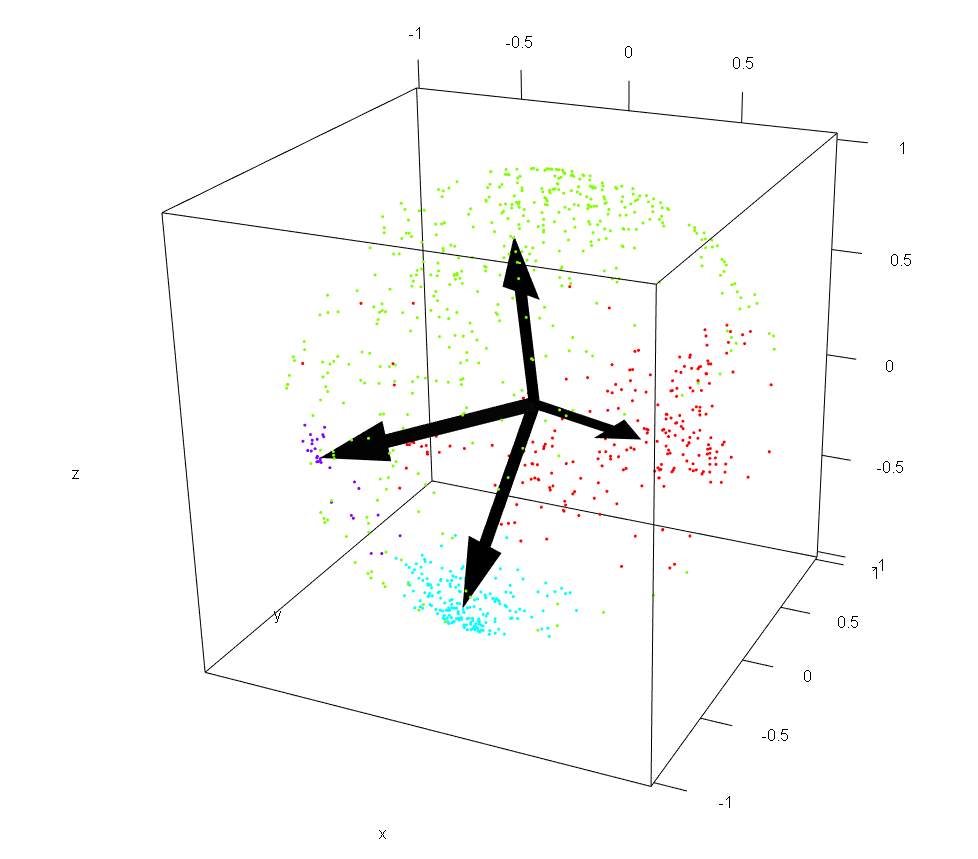
\includegraphics[clip,height= 45mm]{data/cluster_3d.png}
\end{center}
\end{minipage}
\hspace{-0.5cm}
\begin{minipage}{0.5\hsize}
\begin{center}
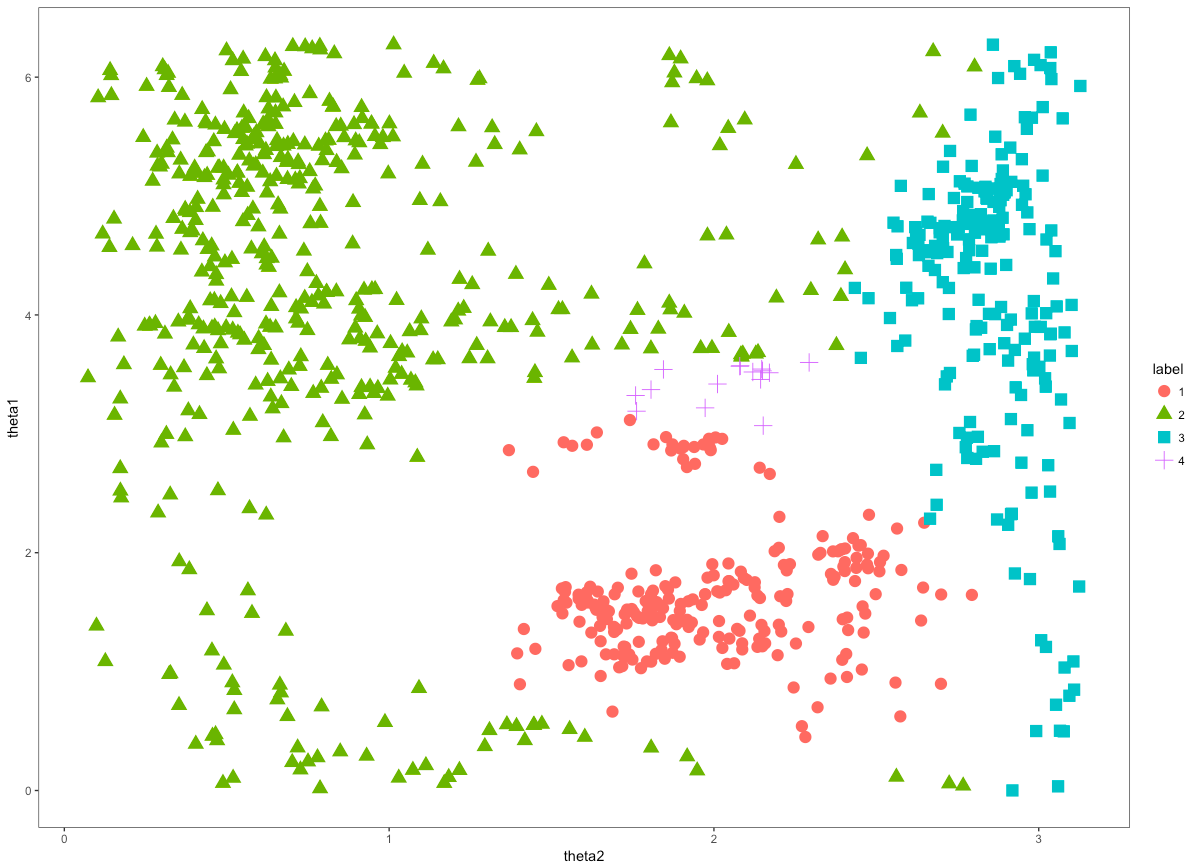
\includegraphics[clip,height= 45mm]{data/cluster_4.png}
\end{center}
\end{minipage}

\end{tabular}
\label{fig2}
\caption{混合分垃による, 球面䞊におけるクラスタリング結果(å·Š), 混合分垃による, 球面䞊の角床$\bm \theta = (\theta_1, \theta_2)^T$におけるクラスタリング結果(右)}
\end{figure}
\end{frame}

\begin{frame}{デヌタ解析(3/3)}
\begin{figure}[tbp]
\begin{center}
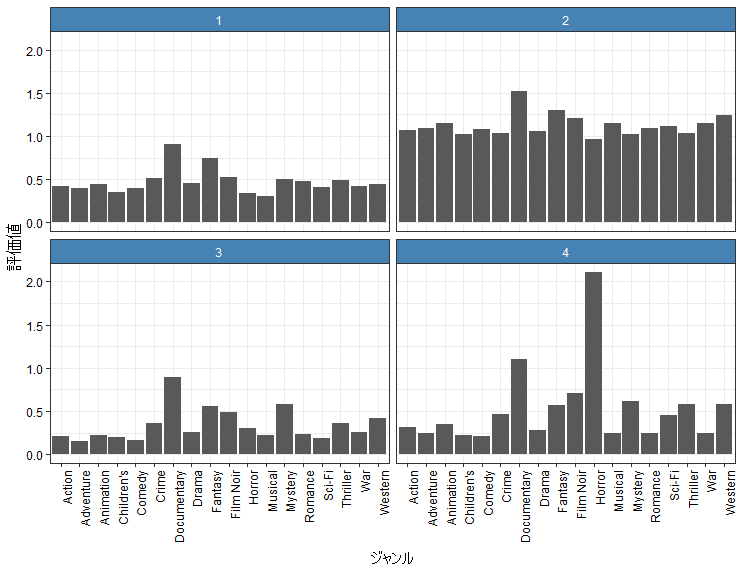
\includegraphics[clip,height= 55mm]{data/cluster_plot.png}
\end{center}
\caption{カテゎリごずのゞャンルぞの平均評䟡倀}
\label{clustergenre}
\end{figure}

\begin{itemize}
	\item カテゎリ2はすべおのゞャンルぞの評䟡倀が高く, その他のカテゎリでは, ゞャンルぞの評䟡倀に差異が珟れた.
\end{itemize}
\end{frame}

%%%%%%%%%%%%%% たずめず今埌の課題 %%%%%%%%%%%%%%%%%
\section{たずめず今埌の課題}
\begin{frame}{たずめず今埌の課題}

\begin{itemize}

\item
䞀般化射圱正芏分垃では任意次元の超球面においお分垃を生成するこずができるので, 次元を圧瞮するこずなく超球面䞊でのクラスタリングに取り組みたい. 

\vspace{0.2cm}
\item
数倀デヌタを球面䞊に配眮し, クラスタリングを行ったが, 超球面䞊でのクラスタリングは䞻にテキストマむニングや画像デヌタに甚いられおいるので, それらのデヌタに察するパラメトリックなクラスタリングを行い, 埓来手法ずの比范を行いたい. 

\end{itemize}

\end{frame}

\section{参考文献}
\begin{frame}{参考文献}

{\scriptsize
\begin{thebibliography}{99}
%\setlength{\itemsep}{-.5zw}
\beamertemplatetextbibitems %参考文献に番号を振る

\bibitem{GPN}
D.Hernandez-Stumpfhauser and F. J. Breidt and Mark J. van der Woerd. (2017). The General Projected Normal Distribution of Arbitrary Dimension: Modeling and Bayesian Inference. {\it Journal of Bayesian Analysis}, Vol. 12, No. 1, pp. 113-133.

\bibitem{PN1}
F. Wang and A. E. Gelfand. (2013). Directional data analysis under the general
projected normal distribution. {\it Statistical Methodology}, Vol.10, pp. 113-127.

\bibitem{PN2}
B. Presnell, S. P. Morrison, and R. C. Littell. (1998). Projected multivariate linear models for
directional data. {\it Journal of the American Statistical Association}, Vol. 443, pp. 1068-1077.

%\bibitem{mvonMF}
%Jalil Taghia and Zhanyu Ma and Arne Leijon. (2014). Bayesian Estimation of the von-Mises Fisher Mixture %Model with Variational Inference. {\it IEEE}, Vol.36, No. 9, pp. 1701-1715.

\bibitem{vonMF}
S. Gopal and Y. Yang. (2014). Von Mises-Fisher Clustering Models. {\it ICML}.

\bibitem{skmeans}
S. Dhillon and S. Modha. (2001). Concept Decompositions for Large Sparse Text Data Using
Clustering. {\it Machine Learning}, Vol. 42, pp. 143-175.

\bibitem{movie}
GroupLensホヌムペヌゞ(http://movielens.org/.) 

\end{thebibliography}
}

\end{frame}

%%%%%%%%%%%%%%付録%%%%%%%%%%%%%%%%付録%%%%%%%%%%%%%%
\backupbegin
\begin{frame}{識別性}
\begin{itemize}
	\item 
	識別性ずは, 異なるパラメヌタにおいお, $p(\theta; \mu_1, \Sigma_1)$ず$p(\theta; \mu_2, \Sigma_2)$が異なるずいうこずである. 射圱正芏分垃は異なるパラメヌタでも同様の確率分垃ずなるこずがあるため, 分散パラメヌタの$1$぀を固定しお, 識別性を保持する.
\end{itemize}

\begin{figure}[htbp]
 \begin{tabular}{c}
 %\hspace{0.5cm}
 \begin{minipage}{0.5\hsize}
  \begin{center}
   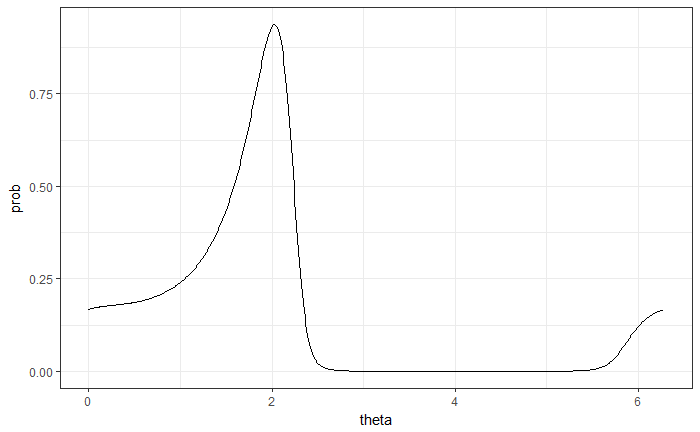
\includegraphics[clip,height= 30mm]{data/pn_sikibetu_real.png}
  \end{center}
 \end{minipage}
 \begin{minipage}{0.5\hsize}
  \begin{center}
 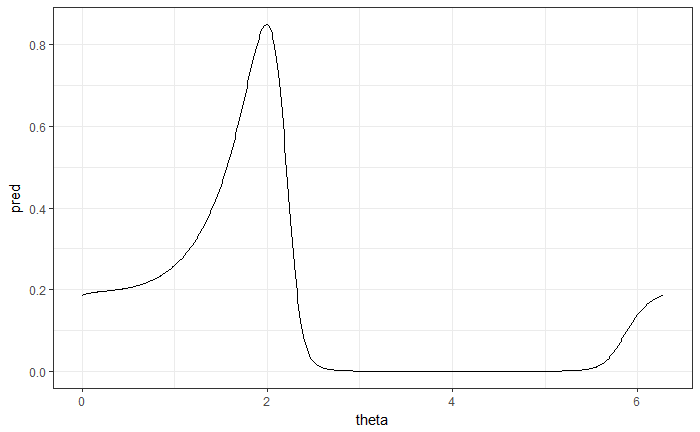
\includegraphics[clip,height= 30mm]{data/pn_sikibetu_pred.png}
  \end{center}
 \end{minipage}
\end{tabular}
\caption{異なるパラメヌタにおける射圱正芏分垃の分垃䟋}
\end{figure}

\end{frame}

\begin{frame}{混合分垃によるクラスタリングの図䟋}

\begin{itemize}
	\item 混合分垃によるクラスタリングでは, $\alpha$をカテゎリ1に, $\beta$をカテゎリ2に分類する.
\end{itemize}

\begin{figure}[tbp]
\begin{center}
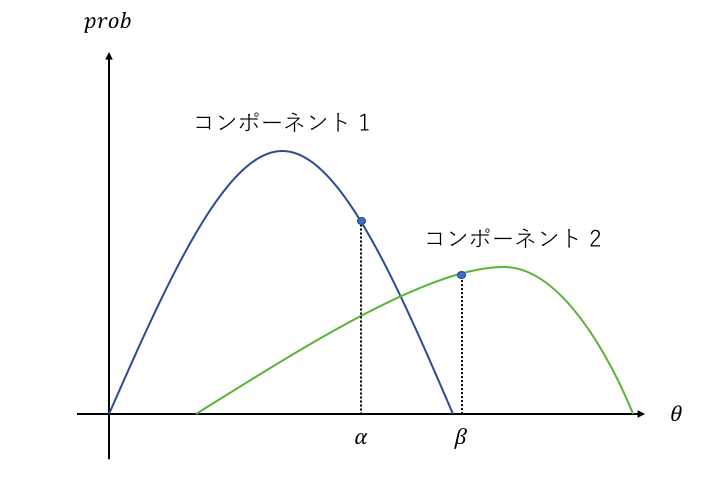
\includegraphics[clip,height= 50mm]{data/mix_cluster.png}
\end{center}
\caption{混合分垃によるクラスタリング分析䟋}
\label{mix_cluster}
\end{figure}

\end{frame}

\begin{frame}{t-SNE(1/2)}

t-SNEは高次元デヌタの次元を圧瞮するアルゎリズムである. このアルゎリズムでは高次元空間における$2$点間の近さを確率分垃ずしお衚珟する. 高次元デヌタ$\bm x$を䜎次元デヌタ$\bm y$に近䌌するずき, 次元圧瞮前の点$x_j$ず点$x_i$の類䌌床を衚す, 条件付確率$P_{j|i}$を甚いお, 同時確率$P_{ij}$を定矩し, 次元圧瞮埌の点$y_j$ず点$y_i$の類䌌床を同時確率$Q_{ij}$によっお定矩する.

\footnotesize
\begin{eqnarray*}
\label{tsne1}
P_{j|i} = \frac{\exp(-\|x_i - x_j\|^2 / 2\sigma_i^2)}{\Sigma_{k \neq i}\exp(-\|x_i - x_k\|^2/ 2\sigma_i^2)},\ 
P_{ij} = \frac{P_{j|i} + P_{i|j}}{2N},\ 
Q_{ij} = \frac{(1 + \|y_i - y_j\|^2)^{-1}}{\Sigma_{k \neq i}(1 + \|y_i - y_k\|^2)^{-1}},
\end{eqnarray*}
\normalsize

\noindent
ここで, $\sigma_i$は点$x_i$を䞭心ずした正芏分垃における, 任意の分散パラメヌタである.
\end{frame}

\begin{frame}{t-SNE(2/2)}

圧瞮前の確率分垃ず圧瞮埌の確率分垃のKL情報量を損倱関数$L$ずしお, $L$が最小になるような$y_i$を求めるこずで, 䜎次元デヌタ$\bm y$を取埗する. 損倱関数$L$を以䞋に瀺す.

\begin{eqnarray*}
\label{tsne3}
L = KL(P || Q) = \Sigma_i \Sigma_j P_{ij} \log \frac{P_{ij}}{Q_{ij}}.
\end{eqnarray*}
\end{frame}

\begin{frame}{MCMC}

マルコフ連鎖で衚されるダむナミクスを甚いお, 䞎えられた確率分垃からのサンプルを埗るアルゎリズムをマルコフ連鎖モンテカルロ法(Markov Chain Monte Carlo Methods)ず呌ぶ.

\begin{itemize}
	\item 
	サンプリング数 : 発生させる各パラメヌタのサンプリング数.
	\vspace{0.2cm}
	\item
	バヌンむン期間 : 各パラヌメヌタにおいお, 収束に芁する期間のこずであり, この期間䞭に埗られたサンプリングは, 平均倀を求める際に含めない.
\end{itemize}
	
\end{frame}


\begin{frame}{HMC(1/2)}

MCMCアルゎリズムの䞀぀である, ハミルトニアン$\cdot$モンテカルロ法(HMC)を甚いお分垃の掚定を行う. ハミルトニアンずはポテンシャル゚ネルギヌ $U(\bm \eta)$ ず運動゚ネルギヌ $V(\bm q)$ の和で定矩される物理量 $H(\bm \eta, \bm q) = U(\bm \eta) + V(\bm q)$ のこずであり. ここで, $\bm q = (q_1, \dots, q_d)^T$ は$\bm \eta$ ず同じ次元のベクトルである. $t$番目のステップにおける, ハミルトニアン方皋匏は以䞋で定矩される. 

\begin{eqnarray*}
\label{HMC}
\frac{d \eta_j(t)}{dt} = \frac{\partial V(\bm q)}{\partial q_j},\ \ \frac{d q_j(t)}{dt} = - \frac{\partial U(\bm \eta)}{\partial \eta_j},
\end{eqnarray*}
\end{frame}

\begin{frame}{HMC(2/2)}

\begin{enumerate}

\item{}
$\eta_j(0), q_j(0)$の初期倀を蚭定する. $\eta_j(0)$は各パラメヌタの事前分垃からの蚭定し, $q_j(0)$は$N(0,M_j)$からランダムサンプリングする. $M_j$ は任意の分散パラメヌタである. 
 
\item{}

以䞋の匏に埓い, $\eta_j, \bm q_j$を曎新する. $\epsilon$は状態倉化のステップ幅を衚す.
\footnotesize
\begin{eqnarray*}
&&q_j(t+\frac{\epsilon}{2}) = q_j(t) - \frac{\epsilon}{2} \frac{\partial U}{\partial \eta_j} (\bm \eta(t)),\ 
\eta_j(t+\epsilon) = \eta_j(t) + \epsilon \frac{q_j(t + \frac{\epsilon}{2})}{M_j},\\ 
&&q_j(t+\epsilon) = q_j(t+\frac{\epsilon}{2}) - \frac{\epsilon}{2} \frac{\partial U}{\partial \eta_j} (\bm \eta(t + \epsilon)),
\end{eqnarray*}
\normalsize

\item{}
埗られたパラメヌタの採択, 棄华を決定する. 䞊蚘のステップで埗られたパラメヌタを$\eta^*_j, q^*_j$ずしお,
珟圚が$t$回目の反埩ずするず, サンプルの棄华率は以䞋の匏で定矩する.

\vspace{-0.5cm}
\begin{eqnarray*}
r_j = \frac{p(\eta^*_j|\theta_j) p(q^*_j)}{p(\eta_j(t-1)|\theta_j) p(q_j(t-1))}.
\end{eqnarray*}

\item{}
䞀様乱数 $u_j \sim U(0,1)$を発生し, $r_j > u_j$ならば, ランダムサンプル $\eta^*_j$を採択し, $r_j < u_j$ならば, $\eta_j(t-1)$を保持する. サンプル数$T$が任意の数に達したずき, MCMCサンプリングを終了する. 

\end{enumerate}

\end{frame}

\begin{frame}{ゞャンルぞの評䟡倀の算出方法(1/2)}
各ナヌザの評䟡倀ず各映画のゞャンル($19$皮類)を甚いお, ナヌザごずに各ゞャンルぞの総評䟡倀を算出する. 各映画には耇数のゞャンルが察応しおいる. ナヌザごずに党おの映画に察しお, 

\begin{equation*}
\mbox{(任意の映画に察する評䟡倀)} \times \mbox{(任意の映画のゞャンル)},
\end{equation*}

\noindent
を算出し, 総和をずるこずで, ナヌザごずに各ゞャンルぞの総評䟡倀を求めた. これらの蚈算は, ナヌザヌ($943$人)$\times$コンテンツ($1682$個)の行列ずコンテンツ($1682$個)$\times$ゞャンル($19$個)の行列の挔算に盞圓しおおり, 省略圢を以䞋に瀺す. 

\footnotesize %匏を小さくする
\begin{equation*}
\label{user_genre_matrix}
\begin{pmatrix} 
5 & 3 & 4 & 3 & \ldots & 0 \\
4 & 0 & 0 & 0 & \ldots & 0 \\
\vdots & \vdots & \vdots & \vdots & \ddots & \vdots \\
0 & 5 & 0 & 0 & \ldots & 0 \\
\end{pmatrix} 
\times
\begin{pmatrix} 
0 & 0 & \ldots & 0 \\
0 & 1 & \ldots & 0 \\
0 & 0 & \ldots & 0 \\
0 & 1 & \ldots & 0 \\
\vdots & \vdots & \ddots & \vdots \\
0 & 0 & \ldots & 0 \\
\end{pmatrix}
=
\begin{pmatrix} 
0 & 95 & \ldots & 4 \\
0 & 17 & \ldots & 0 \\
0 & 17 & \ldots & 0 \\
\vdots & \vdots & \ddots & \vdots \\
0 & 227 & \ldots & 23 \\
\end{pmatrix},
\end{equation*}
\normalsize

\end{frame}

\begin{frame}{ゞャンルぞの評䟡倀の算出方法(2/2)}
埗られたナヌザごずゞャンルぞの評䟡倀から, カテゎリごずのゞャンルぞの評䟡倀を求める. 図\ref{genre_count}に瀺すように, 各ゞャンルは均等に出珟しおいないので, 各ゞャンルの圱響を基準化し, 各コンポヌネントでゞャンルぞの評䟡倀の平均倀を算出する.

\vspace{0.2cm}
\begin{figure}[htbp]
\begin{center}
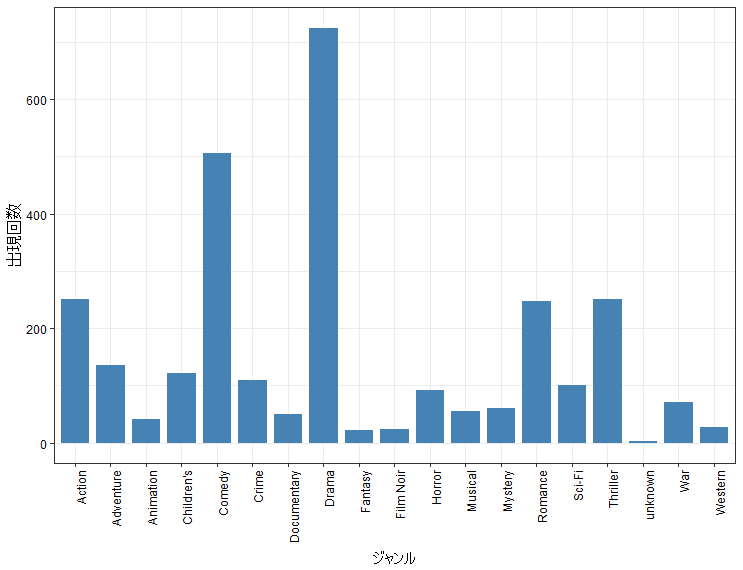
\includegraphics[clip,height= 50mm]{data/genre_count.png}
\end{center}
\caption{コンテンツの各ゞャンルの出珟回数}
\label{genre_count}
\end{figure}
\end{frame}
	
\backupend
\end{document}
